%-*- coding: UTF-8 -*-
% notes.tex
%
\documentclass[UTF8]{article}
\usepackage{geometry}
\geometry{a4paper, centering, scale=0.8}
\usepackage{minted}
\usepackage{hyperref}
\usepackage{indentfirst}    % to indent the first paragraph of a section
\usepackage{graphicx}       % to insert figures


\title{Quickstart Tutorial of NumPy \\
        Learning Notes}
\author{Du Ang \\ \texttt{du2ang233@gmail.com} }
\date{\today}

\begin{document}
\maketitle

\tableofcontents
\newpage

\section{Prerequisites}
Before reading this tutorial you should know a bit of Python. If you would like to refresh your
memory, take a look at the Python tutorial.
\footnote{https://docs.python.org/3/tutorial/}

If you wish to work the examples in this tutorial, you must also have some softwares installed on
your computer. Please see \url{http://scipy.org/install.html} for instructions.

\section{The Basics}
NumPy's main object is the homogeneous multidimensional array. It is a table of elements (usually
numbers), all of the same type, indexed by a tuple of positive integers. In NumPy dimensions are
called \emph{axes}. The number of axes is \emph{rank}.

For example, the coordinates of a point in 3D shape \texttt{[1, 2, 1]} is an array of rank 1,
because it has one axis. That axis has a length of 3. In the example pictured below, the array has
rank 2 (it is 2-dimensional). The first dimension (axis) has a length of 2, the second dimension
has a length of 3.
\begin{minted}{text}
    [[1., 0., 0.],
     [0., 1., 2.]]
\end{minted}

NumPy's array class is called \texttt{ndarray}. It is also known by the alias \texttt{array}. Note
that \texttt{numpy.array} is not the same as the Standard Python Library class \texttt{array.array},
which only handles one-dimensional arrays and offers less functionality. The more important
attributes of an \texttt{ndarray} object are:
\begin{itemize}
    \item \texttt{ndarray.ndim} \\
    the number of axes (dimensions) of the array. In the Python world, the number of dimensions is
    referred to as \emph{rank}.
    \item \texttt{ndarray.shape} \\
    the dimensions of the array. This is a tuple of integers indicating the size of the array in
    each dimension. For a matrix with \emph{n} rows and \emph{m} columns, \texttt{shape} will be
    \texttt{(n, m)}. The length of the \texttt{shape} tuple is therefore the rank, or number of
    dimensions, \texttt{ndim}.
    \item \texttt{ndarray.size} \\
    the total number of elements of the array. This is equal to the product of the elements of
    \texttt{shape}.
    \item \texttt{ndarray.dtype} \\
    an object describing the type of the elements in the array. One can create or specify dtype's
    using standard Python types. Additionally NumPy provides types of its own. \texttt{numpy.int32},
    \texttt{numpy.int16}, and \texttt{numpy.float64} are some examples.
    \item \texttt{ndarray.itemsize} \\
    the size in bytes of each element of the array. For example, an array of elements of type
    \texttt{float64} has \texttt{itemsize} 8 (=64/8), while one of type \texttt{complex32} has
    \texttt{itemsize} 4 (=32/8). It is equivalent to \texttt{ndarray.dtype.itemsize}.
    \item \texttt{ndarray.data} \\
    the buffer containing the actuall elements of the array. Normally, we won't need to use this
    attribute because we will access the elements in an array using indexing facilities.
\end{itemize}

\subsection{An example}
\begin{minted}{numpy}
    >>> import numpy as np
    >>> a = np.arange(15).reshape(3, 5)
    >>> a
    array([[ 0,  1,  2,  3,  4],
           [ 5,  6,  7,  8,  9],
           [10, 11, 12, 13, 14]])
    >>> a.shape
    (3, 5)
    >>> a.ndim
    2
    >>> a.dtype.name
    'int64'
    >>> a.itemsize
    8
    >>> a.size
    15
    >>> type(a)
    <class 'numpy.ndarray'>
    >>> b = np.array([6, 7, 8])
    >>> b
    array([6, 7, 8])
    >>> type(b)
    <class 'numpy.ndarray'>
\end{minted}

\subsection{Array Creation}
There are several ways to create arrays.

For example, you can create an array from a regular Python list or tuple using the \texttt{array}
function. The type of the resulting array is deduced from the type of the elements in the sequence.
\begin{minted}{numpy}
    >>> import numpy as np
    >>> a = np.array([2, 3, 4])
    >>> a
    array([2, 3, 4])
    >>> a.dtype
    dtype('int64')
    >>> b = np.array([1.2, 3.5, 5.1])
    >>> b.dtype
    dtype('float64')
\end{minted}

A frequent error consists in calling \texttt{array} with multiple numeric arguments, rather than
providing a single list of numbers as an argument.
\begin{minted}{numpy}
    >>> a = np.array(1, 2, 3, 4)
    Traceback (most recent call last):
      File "<stdin>", line 1, in <module>
    ValueError: only 2 non-keyword arguments accepted
    >>> a = np.array([1, 2, 3, 4])
\end{minted}

\texttt{array} transforms sequences of sequences into two-dimensional arrays, sequences of
sequences of sequences into three-dimensional arrays, and so on.
\begin{minted}{numpy}
    >>> b = np.array([(1.5, 2, 3), (4, 5, 6)])
    >>> b
    array([[ 1.5,  2. ,  3. ],
       [ 4. ,  5. ,  6. ]])
\end{minted}

The types of the array can also be explicitly specified at creation time:
\begin{minted}{numpy}
    >>> c = np.array([[1, 2], [3, 4]], dtype=complex)
    >>> c
    array([[ 1.+0.j,  2.+0.j],
           [ 3.+0.j,  4.+0.j]])
\end{minted}

Often, the elements of an array are originally unknown, but its size is known. Hence, NumPy offers
several functions to create arrays with innitial placeholder content. These minimize the necessity
of growing arrays, an expensive operation.

The function \texttt{zeros} creates an array full of zeros, the funtion \texttt{ones} creates an
array full of ones, and the funtion \texttt{empty} creates an array whoss initial content is random
and depends on the state of the memory. By default, the dtype of the created array is
\texttt{float64}.
\begin{minted}{numpy}
    >>> np.zeros((3, 4))
    array([[ 0.,  0.,  0.,  0.],
           [ 0.,  0.,  0.,  0.],
           [ 0.,  0.,  0.,  0.]])
    >>> np.ones((2, 3, 4), dtype = np.int16)    # dtype can also be specified
    array([[[1, 1, 1, 1],
            [1, 1, 1, 1],
            [1, 1, 1, 1]],

           [[1, 1, 1, 1],
            [1, 1, 1, 1],
            [1, 1, 1, 1]]], dtype=int16)
    >>> np.empty((2, 3))    # uninitialized, output may vary
    array([[ 0.,  0.,  0.],
           [ 0.,  0.,  0.]])
\end{minted}

To create sequence of numbers, NumPy provides a function analogous to \texttt{range} that returns
arrays instead of lists.
\begin{minted}{numpy}
    >>> np.arange(10, 30, 5)
    array([10, 15, 20, 25])
    >>> np.arange(0, 2, 0.3)    # it accepts float arguments
    array([ 0. ,  0.3,  0.6,  0.9,  1.2,  1.5,  1.8])
\end{minted}

When \texttt{arange} is used with floating point arguments, it is generally not possible to predict
the number of elements obtained, due to the finite floating point of precision. For this reason, it
is usually better to use the function \texttt{linspace} that receives as an arguemnt the nubmer of
elements that we want, instead of the step:
\begin{minted}{numpy}
    >>> from numpy import pi
    >>> # linspace(start, stop, num=50, endpoint=True, retstep=False, dtype=None)
    >>> np.linspace(0, 2, 9)
    array([ 0.  ,  0.25,  0.5 ,  0.75,  1.  ,  1.25,  1.5 ,  1.75,  2.  ])
    >>> x = np.linspace(0, 2*pi, 100)
    >>> f = np.sin(x)
\end{minted}

\subsection{Printing Arrays}
When you print an array, NumPy displays it in a similar way to nested lists, but with the following
layout:
\begin{itemize}
    \item the last axis is printed from left to right
    \item the second-to-last is printed from top to bottom
    \item the rest are also printed from top to bottom, with each slice separated from the next by
    an empty line
\end{itemize}

One-dimensional arrays are then printed as rows, bidimensional as matirces and tridimensional as
lists of matrices.
\begin{minted}{numpy}
    >>> a = np.arange(6)                    # 1d array
    >>> print(a)
    [0 1 2 3 4 5]
    >>>
    >>> b = np.arange(12).reshape(4, 3)     # 2d array
    >>> print(b)
    [[ 0  1  2]
     [ 3  4  5]
     [ 6  7  8]
     [ 9 10 11]]
    >>>
    >>> c = np.arange(24).reshape(2, 3, 4)  # 3d array
    >>> print(c)
    [[[ 0  1  2  3]
      [ 4  5  6  7]
      [ 8  9 10 11]]

     [[12 13 14 15]
      [16 17 18 19]
      [20 21 22 23]]]
\end{minted}

See below to get more details on \texttt{reshape}.

If an array is too large to be printed, NumPy automatically skips the central part of the array and
only prints the corners:
\begin{minted}{numpy}
    >>> print(np.arange(10000))
    [   0    1    2 ..., 9997 9998 9999]
    >>>
    >>> print(np.arange(10000).reshape(100, 100))
    [[   0    1    2 ...,   97   98   99]
     [ 100  101  102 ...,  197  198  199]
     [ 200  201  202 ...,  297  298  299]
     ...,
     [9700 9701 9702 ..., 9797 9798 9799]
     [9800 9801 9802 ..., 9897 9898 9899]
     [9900 9901 9902 ..., 9997 9998 9999]]
\end{minted}

To disable this behaviour and force NumPy to print the entire array, you can change the printing
options using \texttt{set\_printoptions}.
\begin{minted}{numpy}
    >>> np.set_printoptions(threshold='nan')
\end{minted}

\subsection{Basic Operations}
Arithmetic operators on arrays apply \emph{elementwise}. A new array is created and filled with the
result.
\begin{minted}{numpy}
    >>> a = np.array([20, 30, 40, 50])
    >>> b = np.arange(4)
    >>> b
    array([0, 1, 2, 3])
    >>> c = a - b
    >>> c
    array([20, 29, 38, 47])
    >>> b**2
    array([0, 1, 4, 9])
    >>> 10 * np.sin(a)
    array([ 9.12945251, -9.88031624,  7.4511316 , -2.62374854])
    >>> a < 35
    array([ True,  True, False, False], dtype=bool)
\end{minted}

Unlike in many matrix languages, the product operator \texttt{\*} operates elementwise in NumPy
arrays. The matrix product can be performed using the \texttt{dot} function or method:
\begin{minted}{numpy}
    >>> A = np.array([[1, 1],
    ...             [0, 1]])
    >>> B = np.array([[2, 0],
    ...             [3, 4]])
    >>> A * B           # elementwise product
    array([[2, 0],
           [0, 4]])
    >>> A.dot(B)        # matrix product
    array([[5, 4],
           [3, 4]])
    >>> np.dot(A, B)    # another matrix product
    array([[5, 4],
           [3, 4]])
\end{minted}

Some operations, such as \texttt{+=} and \texttt{*=}, act in place to modify an existing array
rather than create a new one.
\begin{minted}{numpy}
    >>> a = np.ones((2, 3), dtype=int)
    >>> b = np.random.random((2, 3))
    >>> a *= 3
    >>> a
    array([[3, 3, 3],
           [3, 3, 3]])
    >>> b += a
    >>> b
    array([[ 3.68582548,  3.15959264,  3.68984824],
           [ 3.67301667,  3.64224267,  3.78424707]])
    >>> a += b      # b is not automatically converted to integer type
    Traceback (most recent call last):
      File "<stdin>", line 1, in <module>
    TypeError: Cannot cast ufunc add output from dtype('float64') to dtype('int64') with
    casting rule 'same_kind'
\end{minted}

When operating with arrays of different types, the type of resulting array corresponds to the more
general or precise one (a behavior known as upcasting).
\begin{minted}{numpy}
    >>> a = np.ones(3, dtype=np.int32)
    >>> b = np.linspace(0, pi, 3)
    >>> b.dtype.name
    'float64'
    >>> c = a + b
    >>> c
    array([ 1.        ,  2.57079633,  4.14159265])
    >>> c.dtype.name
    'float64'
    >>> d = np.exp(c*1j)
    >>> d
    array([ 0.54030231+0.84147098j, -0.84147098+0.54030231j,
           -0.54030231-0.84147098j])
    >>> d.dtype.name
    'complex128'
\end{minted}

Many unary operations, such as computing the sum of all the elements in the array, are implemented
as methods of the \texttt{ndarray} class.
\begin{minted}{numpy}
    >>> a = np.random.random((2, 3))
    >>> a
    array([[ 0.33772353,  0.43252608,  0.36205143],
           [ 0.63473759,  0.01005969,  0.50547396]])
    >>> a.sum()
    2.2825722818751424
    >>> a.min()
    0.010059688136148881
    >>> a.max()
    0.63473759159170229
\end{minted}

By default, these operations apply to the array as though it were a list of numbers, regardless of
its shape. However, by specifying the the \texttt{axis} parameters you can apply an operation along
the specified axis of an array:
\begin{minted}{numpy}
    >>> b = np.arange(12).reshape(3, 4)
    >>> b
    array([[ 0,  1,  2,  3],
           [ 4,  5,  6,  7],
           [ 8,  9, 10, 11]])
    >>> b.sum(axis=0)           # sum of each column
    array([12, 15, 18, 21])
    >>> b.min(axis=1)           # min of each row
    array([0, 4, 8])
    >>>
    >>> b.cumsum(axis=1)        # cumulative sum along each row
    array([[ 0,  1,  3,  6],
          [ 4,  9, 15, 22],
          [ 8, 17, 27, 38]])
\end{minted}

\subsection{Universal Functions}
NumPy provides familiar mathematical functions such as sin, cos, and exp. In NumPy, these are
called ``universal functions'' (\texttt{ufunc}). Within NumPy, these functions operate elementwise
on an array, producting an array as output.
\begin{minted}{numpy}
    >>> B = np.arange(3)
    >>> B
    array([0, 1, 2])
    >>> np.exp(B)
    array([ 1.        ,  2.71828183,  7.3890561 ])
    >>> np.sqrt(B)
    array([ 0.        ,  1.        ,  1.41421356])
    >>> C = np.array([2., -1, 4.])
    >>> np.add(B, C)
    array([ 2.,  0.,  6.])
\end{minted}

\subsection{Indexing, Slicing and Iterating}
\textbf{One-dimensional} arrays can be indexed, sliced and iterated over, much like lists and other
Python sequences.
\begin{minted}{numpy}
    >>> a = np.arange(10)**3
    >>> a
    array([  0,   1,   8,  27,  64, 125, 216, 343, 512, 729])
    >>> a[2]
    8
    >>> a[2:5]
    array([ 8, 27, 64])
    >>> # equivalent to a[0:6:2] = -1000; from start to position 6, exclusive, set
    ... # every 2nd element to -1000
    >>> a[:6:2] = -1000
    >>> a   # reversed a
    array([-1000,     1, -1000,    27, -1000,   125,   216,   343,   512,   729])
    >>> a[ : :-1]
    array([  729,   512,   343,   216,   125, -1000,    27, -1000,     1, -1000])
    >>> for i in a:
    ...     print(i**(1/3.))
    ...
    __main__:2: RuntimeWarning: invalid value encountered in power
    nan
    1.0
    nan
    3.0
    nan
    5.0
    6.0
    7.0
    8.0
    9.0
\end{minted}

\textbf{Multidimensional} arrays can have one index per axis. These indices are given in a tuple
separated by commas:
\begin{minted}{numpy}
    >>> def f(x, y):
    ...     return 10*x+y
    ...
    >>> b = np.fromfunction(f, (5, 4), dtype=int)
    >>> b
    array([[ 0,  1,  2,  3],
           [10, 11, 12, 13],
           [20, 21, 22, 23],
           [30, 31, 32, 33],
           [40, 41, 42, 43]])
    >>> b[2, 3]
    23
    >>> b[0:5, 1]   # each row in the second column
    array([ 1, 11, 21, 31, 41])
    >>> b[ : , 1]   # equivalent to the previous example
    array([ 1, 11, 21, 31, 41])
    >>> b[1:3, : ]  # each column in the second and third row of b
    array([[10, 11, 12, 13],
           [20, 21, 22, 23]])
\end{minted}

When fewer indices are provided than the number of axes, the missing indices are considered
complete slices \texttt{:}
\begin{minted}{numpy}
    >>> b[-1]   # the last row. Equivalent to b[-1, :]
    array([40, 41, 42, 43])
    >>> b[-1, :]
    array([40, 41, 42, 43])
\end{minted}

The expression within brackets in \texttt{b[i]} is treated as an \texttt{i} followed by as many
instances of \texttt{:} as needed to represent the remaining axes. NumPy also allows you to write
this using dots as \texttt{b[i, ...]}.

The \textbf{dots}(\texttt{...}) represent as many colons as needed to produce a complete indexing
tuple. For example, if \texttt{x} is a rank 5 array (i.e., it has 5 axes), then
\begin{itemize}
    \item \texttt{x[1, 2, ...]} is equivalent to \texttt{x[1, 2, :, :, :]}
    \item \texttt{x[..., 3]} to \texttt{x[:, :, :, :, 3]}
    \item \texttt{x[4, ..., 5, :]} to \texttt{x[4, :, :, 5, :]}
\end{itemize}
\begin{minted}{numpy}
    >>> c = np.array([[[0, 1, 2],       # a 3D array (two stacked 2D arrays)
    ...             [10, 12, 13]],
    ...             [[100, 101, 102],
    ...             [110, 112, 113]]])
    >>> c.shape
    (2, 2, 3)
    >>> c[1, ...]                       # same as c[1, :, :] or c[1]
    array([[100, 101, 102],
           [110, 112, 113]])
    >>> c[..., 2]                       # same as c[:, :, 2]
    array([[  2,  13],
           [102, 113]])
\end{minted}

\textbf{Iterating} over multidimensional arrays is done with respect to the first axis:
\begin{minted}{numpy}
    >>> for row in b:
    ...     print(row)
    ...
    [0 1 2 3]
    [10 11 12 13]
    [20 21 22 23]
    [30 31 32 33]
    [40 41 42 43]
\end{minted}

However, if one wants to perform an operation on each element in the array, one can use the
\texttt{flat} attribute which is an iterator over all the elements of the array:
\begin{minted}{numpy}
    >>> for element in b.flat:
    ...     print(element)
    ...
    0
    1
    2
    3
    10
    11
    12
    13
    20
    21
    22
    23
    30
    31
    32
    33
    40
    41
    42
    43
\end{minted}

\section{Shape Manipulation}
\subsection{Changing the shape of an array}
An array has a shape given by the number of elements along each axis:
\begin{minted}{numpy}
    >>> a = np.floor(10*np.random.random((3, 4)))
    >>> a
    array([[ 3.,  4.,  8.,  9.],
           [ 1.,  4.,  1.,  0.],
           [ 1.,  0.,  0.,  1.]])
    >>> a.shape
    (3, 4)
\end{minted}

The shape of an array can  be changed with various commands. Note that the following three commands
all return a modified array, but do not change the original array:
\begin{minted}{numpy}
    >>> a.ravel()       # returns the array, flattened
    array([ 3.,  4.,  8.,  9.,  1.,  4.,  1.,  0.,  1.,  0.,  0.,  1.])
    >>> a.reshape(6, 2) # returns the array with a modified shape
    array([[ 3.,  4.],
           [ 8.,  9.],
           [ 1.,  4.],
           [ 1.,  0.],
           [ 1.,  0.],
           [ 0.,  1.]])
    >>> a.T             # returns the array, transposed
    array([[ 3.,  1.,  1.],
          [ 4.,  4.,  0.],
          [ 8.,  1.,  0.],
          [ 9.,  0.,  1.]])
    >>> a.T.shape
    (4, 3)
    >>> a.shape
    (3, 4)
\end{minted}

The order of the elements in the array resulting from ravel() is normally ``C-style'', that is, the
rightmost index ``changes the fast'', so the element after a[0, 0] is a a[0, 1]. If the array is
reshaped to some other shape, again the array is treated as ``C-style''. NumPy normally creates
arrays stored in this order, so ravel() will usually not need to copy its argument, but if the
array was made by taking slices of another array or created with unusal options, it may need to be
copied. The functions ravel() and reshape() can also be instructed, using an optional argument, to
use FORTRAN-style arrays, in which the leftmost index changes the fastest.

The \texttt{reshape} function returns its argument with a modified shape, whereas the
\texttt{ndarray.resize} method modifies the array itself:
\begin{minted}{numpy}
    >>> a
    array([[ 3.,  4.,  8.,  9.],
           [ 1.,  4.,  1.,  0.],
           [ 1.,  0.,  0.,  1.]])
    >>> a.resize((2, 6))
    >>> a
    array([[ 3.,  4.,  8.,  9.,  1.,  4.],
           [ 1.,  0.,  1.,  0.,  0.,  1.]])
\end{minted}

If a dimension is given as -1 in a reshaping operation, the other dimensions are automatically
calculated:
\begin{minted}{numpy}
    >>> a.reshape(3, -1)
    array([[ 3.,  4.,  8.,  9.],
           [ 1.,  4.,  1.,  0.],
           [ 1.,  0.,  0.,  1.]])
\end{minted}

\subsection{Stacking together different arrays}
Several arrays can be stacked together along different axes:
\begin{minted}{numpy}
    >>> a = np.floor(10*np.random.random((2, 2)))
    >>> a
    array([[ 8.,  3.],
           [ 2.,  4.]])
    >>> b = np.floor(10*np.random.random((2, 2)))
    >>> b
    array([[ 5.,  7.],
           [ 4.,  9.]])
    >>> np.vstack((a, b))
    array([[ 8.,  3.],
           [ 2.,  4.],
           [ 5.,  7.],
           [ 4.,  9.]])
    >>> np.hstack((a, b))
    array([[ 8.,  3.,  5.,  7.],
           [ 2.,  4.,  4.,  9.]])
\end{minted}

The function \texttt{column\_stack} stacks 1D arrays as columns into a 2D array. It is equivalent
to \texttt{vstack} only for 1D arrays:
\begin{minted}{numpy}
    >>> from numpy import newaxis
    >>> np.column_stack((a, b))     # with 2D arrays
    array([[ 8.,  3.,  5.,  7.],
           [ 2.,  4.,  4.,  9.]])
    >>> a = np.array([4., 2.])
    >>> b = np.array([2., 8.])
    >>> a[:, newaxis]               # this allows to have a 2D columns vector
    array([[ 4.],
           [ 2.]])
    >>> np.column_stack((a[:, newaxis], b[:, newaxis]))
    array([[ 4.,  2.],
           [ 2.,  8.]])
    >>> np.vstack((a[:, newaxis], b[:, newaxis]))   # the behavior of vstack is defferent
    array([[ 4.],
          [ 2.],
          [ 2.],
          [ 8.]])
\end{minted}

For arrays of with more than two dimensions, \texttt{hstack} stacks along their second axes,
\texttt{vstack} stacks along their first axes, and concatenate allows for an optional arguments
giving the number of the axis along which the concatenation should happen.

\textbf{Note:} In complex cases, \texttt{r\_} and \texttt{c\_} are useful for creating arrays by
stacking numbers along one axis. They allow the use of range literals (``:'')
\begin{minted}{numpy}
    >>> np.r_[1:4, 0, 4]
    array([1, 2, 3, 0, 4])
\end{minted}

When used with arrays as arguments, \texttt{r\_} and \texttt{c\_} are similar to \texttt{vstack}
and \texttt{hstack} in their default behavior, but allow for an optional argument giving the number
of the axis along which to concatenate.

\subsection{Splitting one array into several smaller ones}
Using \texttt{hsplit}, you can split an array along its horizontal axis, either by specifying the
number of equally shaped arrays to return, or by specifying the columns after which the division
should occur:
\begin{minted}{numpy}
    >>> a = np.floor(10*np.random.random((2, 12)))
    >>> a
    array([[ 1.,  1.,  8.,  0.,  2.,  5.,  6.,  6.,  2.,  3.,  5.,  5.],
           [ 0.,  4.,  8.,  8.,  8.,  5.,  2.,  0.,  8.,  4.,  8.,  7.]])
    >>> np.hsplit(a, 3)         # split a into 3
    [array([[ 1.,  1.,  8.,  0.],
           [ 0.,  4.,  8.,  8.]]), array([[ 2.,  5.,  6.,  6.],
           [ 8.,  5.,  2.,  0.]]), array([[ 2.,  3.,  5.,  5.],
           [ 8.,  4.,  8.,  7.]])]
    >>> np.hsplit(a, (3, 4))    # split a after the third and the fourth column
    [array([[ 1.,  1.,  8.],
           [ 0.,  4.,  8.]]), array([[ 0.],
           [ 8.]]), array([[ 2.,  5.,  6.,  6.,  2.,  3.,  5.,  5.],
           [ 8.,  5.,  2.,  0.,  8.,  4.,  8.,  7.]])]
\end{minted}

\texttt{vsplit} splits along the vertical axis, and \texttt{array\_split} allows one to specify
along which axis to split.

\section{Copies and Views}
When operating and manipulating arrays, their data is sometimes copied into a new array and
sometimes not. This is often a source of confusion for beginers. There are three cases:

\subsection{No Copy at All}
Simple assignments make no copy of array objects or of their data.
\begin{minted}{numpy}
    >>> a = np.arange(12)
    >>> b = a               # no new object is created
    >>> b is a              # a and b are two names for the same ndarray object
    True
    >>> b.shape = 3, 4      # changes the shape of a
    >>> a.shape
    (3, 4)
\end{minted}

Python passes mutable objects as references, so function calls make no copy.
\begin{minted}{numpy}
    >>> def f(x):
    ...     print(id(x))
    ...
    >>> id(a)               # id is a unique identifier of an object
    4369396080
    >>> f(a)
    4369396080
\end{minted}

\subsection{View or Shallow Copy}
Different array objects can share the same data. The \texttt{view} method creates a new array
object that looks at the same data.
\begin{minted}{numpy}
    >>> c = a.view()
    >>> c is a
    False
    >>> c.base is a         # c is a view of the data owned by a
    True
    >>> c.flags.owndata
    False
    >>> c.shape = 2, 6      # a.shape doesn't change
    >>> a.shape
    (3, 4)
    >>> c[0, 4] = 1234      # a's data changes
    >>> a
    array([[   0,    1,    2,    3],
           [1234,    5,    6,    7],
           [   8,    9,   10,   11]])
\end{minted}

Slicing an array returns a view of it:
\begin{minted}{numpy}
    >>> s = a[ : , 1:3]     # spaces added for clarity; could also be written "s = a[:, 1:3]"
    >>> s[:] = 10           # s[:] is a view of s. Note the difference between s=10 and s[:]=10
    >>> a
    array([[   0,   10,   10,    3],
           [1234,   10,   10,    7],
           [   8,   10,   10,   11]])
\end{minted}

\subsection{Deep Copy}
The \texttt{copy} method makes a complete copy of the array and its data.
\begin{minted}{numpy}
    >>> d = a.copy()        # a new ndarray object with new data is created
    >>> d is a
    False
    >>> d.base is a         # d doesn't share anything
    False
    >>> d[0, 0] = 9999
    >>> a
    array([[   0,   10,   10,    3],
           [1234,   10,   10,    7],
           [   8,   10,   10,   11]])
\end{minted}

\subsection{Functions and Methods Overview}
Here is a list of some useful NumPy functions and methods names ordered in categories. See
\emph{Routines} \footnote{https://docs.scipy.org/doc/numpy-dev/reference/routines.html\#routines}
for the full list.
\begin{itemize}
    \item \textbf{Array Creation} \\
    \texttt{arange, array, copy, empty, empty\_like, eye, fromfile, fromfunction, identity,
    linspace, logspace, mgrid, ogrid, ones, ones\_like, r, zeros, zeros\_like}
    \item \textbf{Conversions} \\
    \texttt{ndarray.astype, atleast\_1d, atleast\_2d, atleast\_3d, mat}
    \item \textbf{Manipulations} \\
    \texttt{array\_split, column\_stack, concatenate, diagonal, dsplit, dstack, hsplit, hstack,
    ndarray.item, newaxis, ravel, repeat, reshape, resize, squeeze, swapaxes, take, transpose,
    vsplit, vstack}
    \item \textbf{Questions} \\
    \texttt{all, any, nonzero, where}
    \item \textbf{Ordering} \\
    \texttt{argmax, argmin, argsort, max, min, ptp, searchsorted, sort}
    \item \textbf{Operations} \\
    \texttt{choose, compress, cumprod, cumsum, inner, ndarray.fill, imag, prod, put, putmask, real,
    sum}
    \item \textbf{Basic Statistics} \\
    \texttt{cov, mean, std, var}
    \item \textbf{Basic Linear Algebra} \\
    \texttt{cross, dot, outer, linalg.svd, vdot}
\end{itemize}

\section{Less Basic}
\subsection{Broadcasting rules}
Broadcasting allows universal functions to deal in meaningful way with inputs that do not have
exactly the same shape.

The first rule of broadcasting is that if all input arrays do not have the same number of
dimensions, a ``1'' will be repeatedly prepended to the shapes of the smaller arrays until all the
arrays have the same number of dimensions.

The second rule of broadcasting ensure that arrays with a size of 1 along a particular dimension
act as if they had the size of the array with the largest shape along that dimension. The value of
the array element is assumed to be the same along that dimension for the ``broadcast'' array.

\begin{minted}{numpy}
    >>> a = np.array([[1], [2], [3], [4]])
    >>> a
    array([[1],
           [2],
           [3],
           [4]])
    >>> b = 100
    >>> a + b
    array([[101],
           [102],
           [103],
           [104]])
    >>>
    >>> a = np.array([[1, 2, 3], [4, 5, 6]])
    >>> a
    array([[1, 2, 3],
           [4, 5, 6]])
    >>> b = np.array([100, 200, 300])   # the result is same if b = np.array([[100, 200, 300]])
    >>> b
    array([[100, 200, 300]])
    >>> a + b
    array([[101, 202, 303],
           [104, 205, 306]])
    >>>
    >>> a = np.arange(5).reshape(1, 5)
    >>> a
    array([[0, 1, 2, 3, 4]])
    >>> b = a.T
    >>> b
    array([[0],
           [1],
           [2],
           [3],
           [4]])
   >>> a + b
   array([[0, 1, 2, 3, 4],
          [1, 2, 3, 4, 5],
          [2, 3, 4, 5, 6],
          [3, 4, 5, 6, 7],
          [4, 5, 6, 7, 8]])
\end{minted}

After application of the broadcasting rules, the sizes of all arrays must match. More details can
be found in \emph{Boradcasting}.
\footnote{https://docs.scipy.org/doc/numpy-dev/user/basics.broadcasting.html}

\section{Fancy indexing and index tricks}
NumPy offers more indexing facilities than regular Python sequences. In addition to indexing by
integers and slices, as we saw before, arrays can be indexed by arrays of integers and arrays of
booleans.

\subsection{Indexing with Arrays of Indices}
\begin{minted}{numpy}
    >>> a = np.arange(12)**2            # the first 12 square numbers
    >>> i = np.array([1, 1, 3, 8, 5])   # an array of indices
    >>> a[i]                            # the elements of a at the position i
    array([ 1,  1,  9, 64, 25])
    >>>
    >>> j = np.array([[3, 4], [9, 7]])  # a bidimensional array of indices
    >>> a[j]                            # the same shape as j
    array([[ 9, 16],
           [81, 49]])
\end{minted}

When the indexed array \texttt{a} is multidimensional, a single array of indices refers to the
first dimension of \texttt{a}. The following example shows this behavior by converting an image of
labels into a color image using a palette.
\begin{minted}{numpy}
    >>> palette = np.array( [ [0, 0, 0],
    ...                       [255, 0, 0],
    ...                       [0, 255, 0],
    ...                       [0, 0, 255],
    ...                       [255, 255, 255] ] )
    >>> image = np.array( [ [0, 1, 2, 0],
    ...                     [0, 3, 4, 0] ] )
    >>> palette[image]
    array([[[  0,   0,   0],
            [255,   0,   0],
            [  0, 255,   0],
            [  0,   0,   0]],

           [[  0,   0,   0],
            [  0,   0, 255],
            [255, 255, 255],
            [  0,   0,   0]]])
\end{minted}

We can also give indices for more than one dimension. The arrays of indices for each dimension must
have the same shape.
\begin{minted}{numpy}
    >>> a = np.arange(12).reshape(3, 4)
    >>> a
    array([[ 0,  1,  2,  3],
           [ 4,  5,  6,  7],
           [ 8,  9, 10, 11]])
    >>> i = np.array([[0, 1],   # indices for the first dim of a
    ...               [1, 2]])
    >>> j = np.array([[2, 1],   # indices for the second dim of a
    ...               [3, 3]])
    >>>
    >>> a[i, j]                 # i and j must have equal shape
    array([[ 2,  5],
           [ 7, 11]])
    >>>
    >>> a[i, 2]
    array([[ 2,  6],
           [ 6, 10]])
    >>> a[:, j]                 # i.e., a[ : , j]
    array([[[ 2,  1],
            [ 3,  3]],

           [[ 6,  5],
            [ 7,  7]],

           [[10,  9],
            [11, 11]]])
\end{minted}

Naturally, we can put \texttt{i} and \texttt{j} in a sequence (say a list) and then do the indexing
with the list.
\begin{minted}{numpy}
    >>> l = [i, j]
    >>> a[l]                    # equivalent to a[i, j]
    array([[ 2,  5],
           [ 7, 11]])
\end{minted}

However, we can not do this by putting \texttt{i} and \texttt{j} into an array, because this array
will be interpreted as indexing the first dimension of a.
\begin{minted}{numpy}
    >>> s = np.array([i, j])
    >>> a[s]                    # not what we want
    Traceback (most recent call last):
      File "<stdin>", line 1, in <module>
    IndexError: index 3 is out of bounds for axis 0 with size 3
    >>>
    >>> a[tuple(s)]             # same as a[i, j]
    array([[ 2,  5],
           [ 7, 11]])
\end{minted}

Another common use of indexing with arrays is the search of the maximum value of time-dependent
series:
\begin{minted}{numpy}
    >>> time = np.linspace(20, 145, 5)              # time scale
    >>> data = np.sin(np.arange(20)).reshape(5, 4)  # 4 time-dependent series
    >>> time
    array([  20.  ,   51.25,   82.5 ,  113.75,  145.  ])
    >>> data
    array([[ 0.        ,  0.84147098,  0.90929743,  0.14112001],
           [-0.7568025 , -0.95892427, -0.2794155 ,  0.6569866 ],
           [ 0.98935825,  0.41211849, -0.54402111, -0.99999021],
           [-0.53657292,  0.42016704,  0.99060736,  0.65028784],
           [-0.28790332, -0.96139749, -0.75098725,  0.14987721]])
    >>>
    >>> ind = data.argmax(axis=0)                   # index of the maxima for each series
    >>> ind
    array([2, 0, 3, 1])
    >>>
    >>> time_max = time[ind]                        # time corresponding to the maxima
    >>> # data_max = data[ind, xrange(data.shape[1])]    # python2 codes
    >>> data_max = data[ind, range(data.shape[1])]  # => data[ind[0], 0], data[ind[1], 1], ...
    >>> time_max
    array([  82.5 ,   20.  ,  113.75,   51.25])
    >>> data_max
    array([ 0.98935825,  0.84147098,  0.99060736,  0.6569866 ])
    >>> data_max = data[ind, range(data.shape[1])]
    >>> time_max
    array([  82.5 ,   20.  ,  113.75,   51.25])
    >>> data_max
    array([ 0.98935825,  0.84147098,  0.99060736,  0.6569866 ])
    >>> np.all(data_max == data.max(axis=0))
    True
\end{minted}

You can also use indexing with arrays as a target to assign to:
\begin{minted}{numpy}
    >>> a = np.arange(5)
    >>> a
    array([0, 1, 2, 3, 4])
    >>> a[[1, 3, 4]] = 0
    >>> a
    array([0, 0, 2, 0, 0])
\end{minted}

However, when the list of indices contains repetitions, the assignment is done several times,
leaving behind the last value:
\begin{minted}{numpy}
    >>> a = np.arange(5)
    >>> a
    array([0, 1, 2, 3, 4])
    >>> a[[0, 0, 2]] = [1, 2, 3]
    >>> a
    array([2, 1, 3, 3, 4])
\end{minted}

This is reasonable enough, but watch out if you want to use Python's \texttt{+=} construct, as it
may not do what you expect:
\begin{minted}{numpy}
    >>> a = np.arange(5)
    >>> a
    array([0, 1, 2, 3, 4])
    >>> a[[0, 0, 2]] += 1
    >>> a
    array([1, 1, 3, 3, 4])
\end{minted}

Even though 0 occurs twice in the list of indices, the 0th element is only incremented once. This
is because Python requires ``a += 1'' to be equivalent to ``a = a + 1''.

\subsection{Indexing with Boolean Arrays}
When we index arrays with arrays of (integer) indices we are providing the list of indices to pick.
With boolean indices the approach is different; we expectly choose which items in the array we want
and which ones we don't.

The most natural way one can think of for boolean indexing is to use boolean arrays that have
\emph{the same shape} as the original array:
\begin{minted}{numpy}
    >>> a = np.arange(12).reshape(3, 4)
    >>> b = a > 4
    >>> b           # b is a boolean with a's shape
    array([[False, False, False, False],
           [False,  True,  True,  True],
           [ True,  True,  True,  True]], dtype=bool)
    >>> a[b]        # 1d array with the selected elements
    array([ 5,  6,  7,  8,  9, 10, 11])
\end{minted}

This property can be very useful in assignments:
\begin{minted}{numpy}
    >>> a[b] = 0    # all elements of 'a' higher than 4 become 0
    >>> a
    array([[0, 1, 2, 3],
           [4, 0, 0, 0],
           [0, 0, 0, 0]])
\end{minted}

You can look at the following example to see how to use boolean indexing to generate an image of
the Mandelbrot set:
\begin{minted}{numpy}
    import numpy as np
    import matplotlib.pyplot as plt


    def mandelbrot(h, w, maxit=20):
        """Returns an image of the Mandelbrot fractal of size (h,w)."""

        y, x = np.ogrid[-1.4:1.4:h * 1j, -2:0.8:w * 1j]
        c = x + y * 1j
        z = c
        divtime = maxit + np.zeros(z.shape, dtype=int)

        for i in range(maxit):
            z = z ** 2 + c
            diverge = z * np.conj(z) > 2 ** 2       # who is diverging
            div_now = diverge & (divtime == maxit)  # who is diverging now
            divtime[div_now] = i                    # note when
            z[diverge] = 2                          # avoid diverging too much

        return divtime


    plt.imshow(mandelbrot(400, 400))
    plt.show()
\end{minted}
(This code should be interpreted by Python 2, out of interactive mode)

\begin{figure}[ht]
    \centering
    \includegraphics[scale=0.6]{mandelbrot.png}
    \caption{Mandelbrot fractal of size (400, 400)}
\end{figure}

The second way of indexing with booleans is more similar to integer indexing; for each dimension of
the array we give a 1D boolean array selecting the slices we want:
\begin{minted}{numpy}
    >>> a = np.arange(12).reshape(3, 4)
    >>> a
    array([[ 0,  1,  2,  3],
           [ 4,  5,  6,  7],
           [ 8,  9, 10, 11]])
    >>> b1 = np.array([False, True, True])          # first dim selection   ==> [1, 2]
    >>> b2 = np.array([True, False, True, False])   # second dim selection  ==> [0, 2]
    >>>
    >>> a[b1, :]                # selecting rows
    array([[ 4,  5,  6,  7],
           [ 8,  9, 10, 11]])
    >>>
    >>> a[b1]                   # same thing
    array([[ 4,  5,  6,  7],
           [ 8,  9, 10, 11]])
    >>>
    >>> a[:, b2]                # selecting columns
    array([[ 0,  2],
           [ 4,  6],
           [ 8, 10]])
    >>> a[b1, b2]               # a werid thing to do, b1 = [1, 2], b2 = [0, 2]
    array([ 4, 10])
\end{minted}
Note that the length of the 1D boolean array must coincide with the length of the dimension (or
axis) you want to slice. In the previous example, \texttt{b1} is a 1-rank array with length 3 (the
number of \emph{rows} in \texttt{a}), and \texttt{b2} (of length 4) is suitable to index the 2nd
rank (columns) of \texttt{a}.
\footnote{https://stackoverflow.com/questions/9883098/}

\subsection{The ix\_() function}
The \texttt{ix\_} function can be used to combine different vectors so as to obtain the result for
each n-uplet. For example, if you want to compute all the a + b * c for triplets taken from each of
the vectors a, b and c:
\begin{minted}{numpy}
    >>> a = np.array([2, 3, 4, 5])
    >>> b = np.array([8, 5, 4])
    >>> c = np.array([5, 4, 6, 8, 3])
    >>> ax, bx, cx = np.ix_(a, b, c)
    >>> ax
    array([[[2]],

           [[3]],

           [[4]],

           [[5]]])
    >>> bx
    array([[[8],
            [5],
            [4]]])
    >>> cx
    array([[[5, 4, 6, 8, 3]]])
    >>> ax.shape, bx.shape, cx.shape
    ((4, 1, 1), (1, 3, 1), (1, 1, 5))
    >>> result = ax + bx * cx
    >>> result
    array([[[42, 34, 50, 66, 26],
            [27, 22, 32, 42, 17],
            [22, 18, 26, 34, 14]],

           [[43, 35, 51, 67, 27],
            [28, 23, 33, 43, 18],
            [23, 19, 27, 35, 15]],

           [[44, 36, 52, 68, 28],
            [29, 24, 34, 44, 19],
            [24, 20, 28, 36, 16]],

           [[45, 37, 53, 69, 29],
            [30, 25, 35, 45, 20],
            [25, 21, 29, 37, 17]]])
    >>> result[3, 2, 4]
    17
    >>> a[3] + b[2] * c[4]
    17
\end{minted}

You could also implement the reduce as follows:
\begin{minted}{numpy}
    >>> def ufunc_reduce(ufct, *vectors):
    ...     vs = np.ix_(*vectors)
    ...     r = ufct.identity
    ...     for v in vs:
    ...         r = ufct(r, v)
    ...     return r
\end{minted}
and then use it as:
\begin{minted}{numpy}
    >>> ufunc_reduce(np.add, a, b, c)
    array([[[15, 14, 16, 18, 13],
            [12, 11, 13, 15, 10],
            [11, 10, 12, 14,  9]],

           [[16, 15, 17, 19, 14],
            [13, 12, 14, 16, 11],
            [12, 11, 13, 15, 10]],

           [[17, 16, 18, 20, 15],
            [14, 13, 15, 17, 12],
            [13, 12, 14, 16, 11]],

           [[18, 17, 19, 21, 16],
            [15, 14, 16, 18, 13],
            [14, 13, 15, 17, 12]]])
\end{minted}

The advantage of this version of reduce compared to the normal \texttt{ufunc.reduce} is that it
makes use of the Broadcasting Rules in order to avoid creating an argument array the size of the
output times the number of vectors.

\subsection{Indexing with strings}
See \emph{Structured arrays}.
\footnote{https://docs.scipy.org/doc/numpy-dev/user/basics.rec.html\#structured-arrays}

\section{Linear Algebra}
Work in progress. Basic linear algebra to be included here.

\subsection{Simple Array Operations}
See \texttt{linalg.py} in numpy folder for more.
\begin{minted}{numpy}
    >>> import numpy as np
    >>> a = np.array([[1.0, 2.0], [3.0, 4.0]])
    >>> print(a)
    [[ 1.  2.]
     [ 3.  4.]]
    >>> a.transpose()
    array([[ 1.,  3.],
           [ 2.,  4.]])
    >>> np.linalg.inv(a)
    array([[-2. ,  1. ],
           [ 1.5, -0.5]])
    >>> u = np.eye(2)               # unit 2x2 matrix; "eye" represents "I"
    >>> u
    array([[ 1.,  0.],
           [ 0.,  1.]])
    >>> j = np.array([[0.0, -1.0], [1.0, 0.0]])
    >>> np.dot(j, j)                # matrix product
    array([[-1.,  0.],
           [ 0., -1.]])
    >>> np.trace(u)                 # trace
    2.0
    >>> y = np.array([[5.], [7.]])
    >>> np.linalg.solve(a, y)       # solve the linear matrix equation `ax = y`
    array([[-3.],
           [ 4.]])
    >>> np.linalg.eig(j)            # eigenvector
    (array([ 0.+1.j,  0.-1.j]), array([[ 0.70710678+0.j        ,  0.70710678-0.j        ],
           [ 0.00000000-0.70710678j,  0.00000000+0.70710678j]]))
\end{minted}
\begin{minted}{text}
    Parameters:
        square matrix
    Returns
        The eigenvalues, each repeated according to its multiplicity.
        The normalized (unit "length") eigenvectors, such that the column ``v[:, i]`` is the
        eigenvector corresponding to the eigenvalue ``w[i]``.
\end{minted}

\section{Tricks and Tips}
Here we give a list of short and useful tips.

\subsection{``Automatic'' Reshaping}
To change the dimensions of an array, you can omit one of the sizes which will then be deduced
automatically:
\begin{minted}{numpy}
    >>> a = np.arange(30)
    >>> a.shape = 2, -1, 3      # -1 means "whatever is needed"
    >>> a.shape
    (2, 5, 3)
    >>> a
    array([[[ 0,  1,  2],
            [ 3,  4,  5],
            [ 6,  7,  8],
            [ 9, 10, 11],
            [12, 13, 14]],

           [[15, 16, 17],
            [18, 19, 20],
            [21, 22, 23],
            [24, 25, 26],
            [27, 28, 29]]])
\end{minted}

\subsection{Vector Stacking}
How do we construct a 2D array from a list of equally-sized row vectors? In MATLAB this is quite
easy: if \texttt{x} and \texttt{y} are two vectors of the same length you only need to do
\texttt{m = [x; y]}. In NumPy this works via the functions \texttt{column\_stack}, \texttt{dstack},
\texttt{hstack} and \texttt{vstack}, depending on the dimension in which the stacking is to be
done. For example:
\begin{minted}{numpy}
    >>> x = np.arange(0, 10, 2)     # x = ([0, 2, 4, 7, 8])
    >>> y = np.arange(5)            # y = ([0, 1, 2, 3, 4])
    >>> m = np.vstack([x, y])
    >>> m
    array([[0, 2, 4, 6, 8],
       [0, 1, 2, 3, 4]])
    >>> xy = np.hstack([x, y])
    >>> xy
    array([0, 2, 4, 6, 8, 0, 1, 2, 3, 4])
\end{minted}

The logic behind those functions in more than two dimensions can be strange. See also \emph{NumPy
for MATLAB users} \footnote{https://docs.scipy.org/doc/numpy-dev/user/numpy-for-matlab-users.html}

\subsection{Histograms}
The NumPy \texttt{histogram} function applied to an array returns a pair of vectors: the histogram
of the array and the vector of bins. Beware: \texttt{matplotlib} also has a function to build
hisograms (called \texttt{hist}, as in MATLAB) that differs from the one in NumPy. The main
difference is that \texttt{pylab.hist} plots the histogram automatically, while
\texttt{numpy.histogram} only generates the data.
\begin{minted}{numpy}
    import numpy as np
    import matplotlib.pyplot as plt

    # Build a vector of 10000 normal deviates with variance 0.5^2 and mean 2
    mu, sigma = 2, 0.5
    v = np.random.normal(mu, sigma, 10000)
    # Plot a normalized histogram with 50 bins
    plt.hist(v, bins=50, normed=1)      # matplotlib version (plot)
    plt.show()

    # Compute the histogram with numpy and then plot it
    (n, bins) = np.histogram(v, bins=50, normed=True)   # NumPy version (no plot)
    plt.plot(.5 * (bins[1:] + bins[:-1]), n)
    plt.show()
\end{minted}

\begin{figure}[ht]
    \centering
    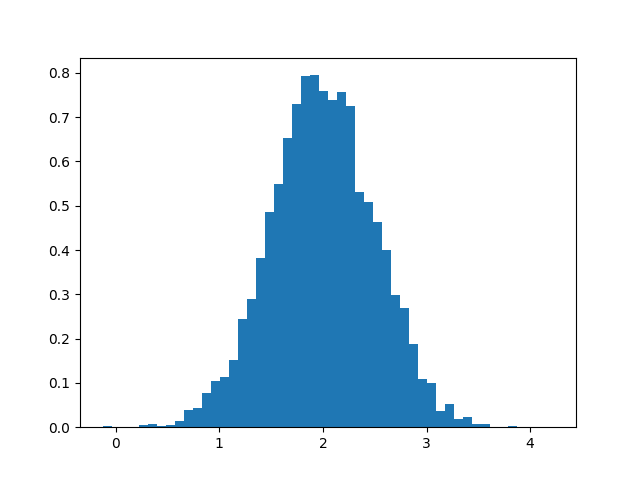
\includegraphics[scale=0.6]{hist_matplotlib.png}
    \caption{The \texttt{matplotlib} version of histogram}
\end{figure}

\begin{figure}[ht]
    \centering
    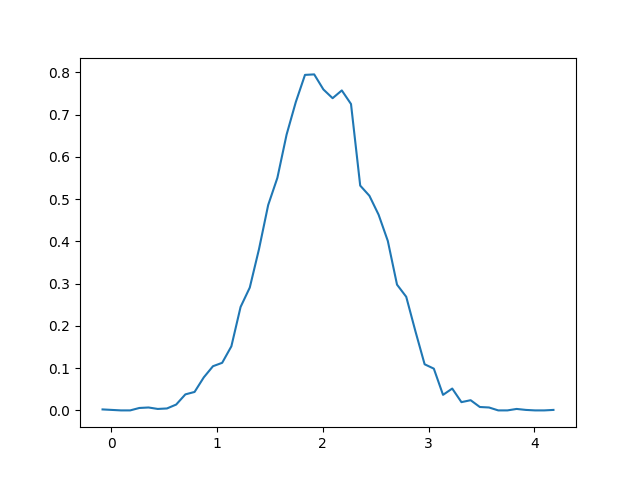
\includegraphics[scale=0.6]{hist_numpy.png}
    \caption{The NumPy version of histogram}
\end{figure}















\end{document}
